上一章把``一个变量有多不确定''变成了一个可以计算的数。可实际工作里很少有单变量的问题：手上永远是一张多列的表，问题永远是列与列之间的事——这一列能替另一列省下多少存储，观测了这一列之后那一列还剩多少悬念，把原始数据加工一遍会不会丢掉要紧的东西。

这一章的共同困难只有一句：把两个变量之间共享的那部分不确定性，变成一个可以加减的量。

\begin{center}
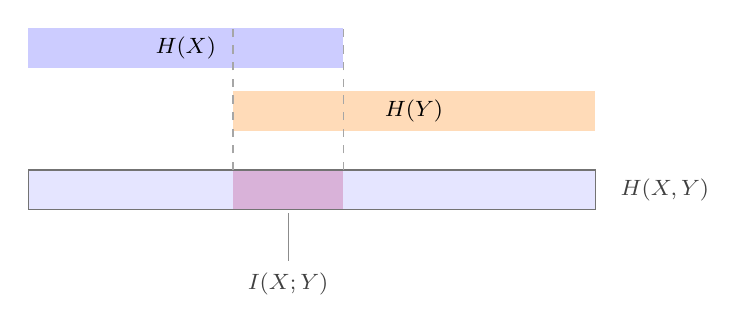
\begin{tikzpicture}[x=1cm,y=1cm,font=\small]
  \fill[blue!20] (0,2.0) rectangle (4.0,2.5);
  \node[font=\footnotesize] at (2.0,2.25) {\(H(X)\)};
  \fill[orange!28] (2.6,1.2) rectangle (7.2,1.7);
  \node[font=\footnotesize] at (4.9,1.45) {\(H(Y)\)};
  \fill[blue!10] (0,0.2) rectangle (7.2,0.7);
  \fill[violet!30] (2.6,0.2) rectangle (4.0,0.7);
  \draw[black!55] (0,0.2) rectangle (7.2,0.7);
  \node[font=\footnotesize,right,black!75] at (7.4,0.45) {\(H(X,Y)\)};
  \draw[black!35,dashed] (2.6,0.7) -- (2.6,2.5);
  \draw[black!35,dashed] (4.0,0.7) -- (4.0,2.5);
  \draw[black!45] (3.3,0.15) -- (3.3,-0.45);
  \node[font=\footnotesize,black!75] at (3.3,-0.75) {\(I(X;Y)\)};
\end{tikzpicture}

\emph{把两个熵首尾相接地摆，重叠的那一段被数了两次。联合熵是并起来的长度，重叠本身就是互信息。分别给两列做存储预算之所以偏大，正是因为这一段付了两遍钱。}
\end{center}

四篇沿着这张图往下走，各自要立起来的判断是：

\begin{itemize}
\tightlist
\item \hyperref[sec:07-Information-Theory/02-Joint-Information/01]{``联合熵、条件熵与链式法则''}：条件熵是``知道 \(Y\) 之后 \(X\) 还剩多少不确定''；链式法则 \(H(X,Y)=H(X)+H(Y\given X)\) 说的是信息可以分步获取而总量不变，与获取顺序无关。
\item \hyperref[sec:07-Information-Theory/02-Joint-Information/02]{``互信息是依赖，也是对不确定性的减少''}：互信息对称、非负，且只有在独立时才为零。这一条让它比相关系数强得多——相关系数只看得见线性关系。
\item \hyperref[sec:07-Information-Theory/02-Joint-Information/03]{``条件互信息与 Markov 结构''}：控制第三个变量可能让依赖消失，也可能让依赖凭空出现；两圆图的直觉到三个变量就失效。
\item \hyperref[sec:07-Information-Theory/02-Joint-Information/04]{``数据处理不等式与充分表示''}：\(X\to Y\to Z\) 时 \(I(X;Z)\le I(X;Y)\)。加工不会增加信息，能改善的只是信息的可提取性。
\end{itemize}

第一篇和第二篇是主线，读完就能开始用；第三篇与\hyperref[sec:05-Probability/02-Conditional-Probability/04]{``条件独立与信息结构''}里的混杂与碰撞结构直接对上，那一篇读过的话这里会很快；第四篇是特征工程和表示学习的信息论底座，也是本章在工程上兑现最多的一篇。

最后留一句贯穿全章的提醒。这些量刻画的都是统计依赖，不是因果影响。互信息高可以来自直接作用，也可以来自共同原因，还可以来自你只看了被筛选过的样本。信息论能把关联的强弱算准，至于这个关联为什么存在，得另找依据。
